\section{C’est dans la boite}


\subsection{Au rapport !}
Nos héros quittant Jebble son contacté par leur faction.

\subsubsection{Empire}
\begin{quotebox}
    \nameref{sec:garan-keggle}: Au rapport~! Comment avancent vos recherches sur l’artefact~?
\end{quotebox}
Les joueurs racontent\ldots
\begin{quotebox}
    \nameref{sec:garan-keggle}: La "Boite de Jebble"\ldots Ça ne me dit rien~! Mais allez voir \nameref{sec:fane-peturri} sur \textbf{Muunilinst}, c’est un historien de l’Empire, ami de notre Empereur, il pourra certainement vous aider. Je vais le prévenir de votre visite et je vous transfère ses coordonnées.
\end{quotebox}

Les héros se rendent donc sur \textbf{Muunilinst} (normalement) et rencontrent \nameref{sec:fane-peturri}. Ce dernier les invite chez lui, leur offre le thé et les reçoit bien.
\begin{quotebox}
    \nameref{sec:fane-peturri}: Garan m’a prévenu de votre arrivée, mais il ne m’a pas dit quel était le but de votre visite~? En quoi puis-je aider l’empire~?
\end{quotebox}
Les héros devraient donc lui parler de la fameuse boite de Jebble qui est en réalité \nameref{sec:oubliette-de-dreypa}.

\begin{quotebox}
    \nameref{sec:fane-peturri}: Il me semblait bien qu’il y avait un rapport entre l’oubliette et cette Boite~! Il y a quelque temps, suite à une réquisition d’\oe{uvres} d’art pour le compte de l’Empire, je suis tombé sur un enregistrement holo qui parlait de cette boite. D’après ce que disait l’enregistrement, mais il date maintenant de plusieurs mois, la \textbf{Boite de Jebble} se trouve sur le \nameref{sec:uhumele} un cargo qui verse dans le commerce et la contrebande de babioles diverses. Son capitaine, \nameref{sec:schurk-heren} est un Yarkora qui se méfie de tout le monde en général et en particulier de l’Empire. Dites-lui que vous êtes des amis de "\textbf{\nameref{sec:uhumele-janks}}" mais il n’est pas idiot donc prenez ce dossier sur Janks et étudiez le avant de vous faire passer pour ses amis.

    Le dernier port d’attache que je lui connais est \textbf{Pizkoss}, il est certainement en train de dépenser ses crédits chez \nameref{sec:queen-jool}.
\end{quotebox}

\subsubsection{Rebelion}
\begin{quotebox}
    \nameref{sec:lindi-dangon}: Bonjour, je viens aux nouvelles, comment se passe la recherche de l’artéfact~? Vous avez besoin de quelque chose~?
\end{quotebox}

Les joueurs racontent\ldots

\begin{quotebox}
    \nameref{sec:lindi-dangon}: La \textbf{Boite de Jebble}, ça me dit quelque chose, attendez une seconde\ldots 

    \textit{Lindi disparaît de l’écran un instant puis revient}

    \nameref{sec:lindi-dangon}: Effectivement, un Jedi en parle dans un de ses rapports. \nameref{sec:dass-jennir}, il n’est pas très précis dans son rapport, mais vous devriez aller le voir. Il est en retraite sur \textbf{Muunilinst}. Je vous fais suivre les coordonnées où vous le trouverez, soyez respectueux et diplomates~! Rappelez-vous que c’est un Jedi~!
\end{quotebox}

Les héros se rendent donc sur \textbf{Muunilinst} (normalement) pour rencontrer \nameref{sec:dass-jennir}. Dass Jennir se montre tout d’abord froid et distant
\begin{quotebox}
    \nameref{sec:dass-jennir}: C’est pour quoi~? Si c’est encore pour réparer votre moissonneuse, revenez plus tard, je suis occupé là.
\end{quotebox}

Aux héros de se montrer diplomate pour l’amadouer~! Quand c’est fait. Ils lui parlent de la Boite de Jebble. En entendant ce nom, le visage de Dass Jennir marque un sentiment de souffrance et de regret. C’est manifestement un souvenir douloureux pour lui.
\begin{quotebox}
    \nameref{sec:dass-jennir}: Oui, je me souviens de ça~! Je ne l’ai pas vu personnellement, mais elle faisait partie de l’inventaire de l’\nameref{sec:uhumele} quand je suis passé à son bord pour une mission. L’équipage du vaisseau avait à son bord cette chose, aux dernières nouvelles ils partaient sur \textbf{Pizkoss} pour tenter de trouver un acheteur pour cette cargaison.

    Vous devez savoir que déjà à l’époque, l’Empire recherchait ardemment cette cargaison, c’est d’ailleurs ce qui explique qu’il ne l’ai toujours pas revendue. 

    Le capitaine du cargo s’appelle \nameref{sec:schurk-heren} je vais vous dire où le trouver sur \textbf{Pizkoss} mais je ne viendrais pas avec vous, j’en ai fini avec tout ça. Habituellement, \nameref{sec:schurk-heren} dépense ses crédits chez \nameref{sec:queen-jool} quand il fait escale à \textbf{Pizkoss}.
\end{quotebox}

\newpage
\subsection{Pizkoss’ Paradise}
Pizkoss est un Monde du Noyau. En tant que tel, le commerce y est très prospère et on y retrouve à peu près toutes les races possibles. Toutes sortes de transaction et ont lieu des plus légales aux plus douteuses. En tant que planète du noyau elle est surveillée par l’Empire.

\nameref{sec:queen-jool} est la propriétaire d’une cantina libertine sur \textbf{Pizkoss}, le \textbf{Paradise}. C’est un club "select" où l’on ne rentre que sur invitation. Il ne faut pas chercher à rentrer de force au risque de se faire expulser violemment et d’attirer par la même l’attention de l’Empire. Diplomatie et astuce (déguisement, soudoiement, propositions indécentes \ldots) sont de rigueur. Une fois à l’intérieur, attention de ne pas faire de vagues~! Au moindre problème, vigiles et \nameref{sec:storm-trooper}s débarquent et enferment tout le monde.\\

\noindent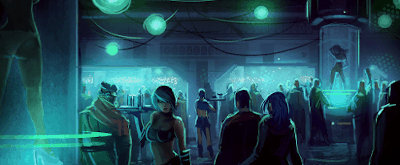
\includegraphics[width=\linewidth]{_img/places/paradise-club.jpg}\\

\'A l’intérieur la salle se présente comme un stripbar classique. Un bar sur la droite, une estrade au fond avec un podium qui avance sur la moitié de la pièce. Des îlots plus privés tout au tour et des salons privatif sur la gauche. 

Les héros ne savent pas à quoi ressemble \nameref{sec:schurk-heren} ils n’ont que son nom, à eux de le retrouver. En vrai il se trouve dans l’un des salons privés où il profite d’une danse avec \textbf{Na’tuna}, une charmante Twi’lek en tenue légère.

Quand les héros rentrent dans le salon, Schurk est un peu surpris, Na’Tuna reste imperturbable, professionnalisme avant tout.

\begin{quotebox}
    \nameref{sec:schurk-heren}: Ben faut pas vous gêner~! Décidément tout se perd, les bonnes manières y compris~! Je ne sais pas ce que vous me voulez mais vous ne pensez pas que ça peut attendre que la dame est terminée~?
\end{quotebox}

Gérez Schurk en fonction du comportement de vos héros, quand ils se mettent à discuter~:

\begin{quotebox}
    \nameref{sec:schurk-heren}: Bon, maintenant que l’on est entre nous, en quoi puis-je vous aider ?\\
    \textit{\textbf{Joueurs}}: \ldots\\
    \nameref{sec:schurk-heren}: Humm, alors comme ça cet inestimable et antique coffre vous intéresse ? C’est fâcheux, figurez-vous que je viens tout juste de le promettre à un client fortuné. Il serait vraiment très déçu si je lui faisais faux bon.\\
    \textit{\textbf{Joueurs}}: \ldots\\
    \nameref{sec:schurk-heren}: Cependant vous m’êtes sympathique~! Il se pourrait que je vous dise où se trouve la cargaison. Si vous êtes assez rapide, vous pourrez la récupérer avant mon autre client. Je n’ai pas encore rencontré mon client pour la transaction, ça vous laisse le temps de me rendre un petit service.\\
    \textit{\textbf{Joueurs}}: \ldots \\
    \nameref{sec:schurk-heren}: Mais vous êtes des amis de \textit{[\textbf{Dass Jennir}|\textbf{Janks}]}, je ne me vois pas vous refuser ça~! Il se trouve que je n’ai pas une confiance aveugle en ce client. Il est connu pour être un criminel et je m’attends à ce qu’il essaye de me doubler. Dans ces conditions, je vous propose d’assister à la transaction de loin. Si ça tourne mal, on se débarrasse de lui et je vous fais la cargaison à prix d’ami.

    Si tout se passe bien, vous connaîtrez l’emplacement de la cargaison et n’aurez qu’a vous y rendre avant eux. C’est ce que je peux vous proposer de mieux.
\end{quotebox}

Peu importe le prix que vous négocierez avec les héros il n’y aura jamais besoin de le payer.
\begin{paperbox}{Songes d’Uhumele}
    \'A noter que si vos héros ont fait le scénar \citetitle{swr-songes-uhumele}, ils connaissent les membres de l’Uhumele ainsi que leur aventure avec \nameref{sec:dass-jennir} et ils ont le droit d’en jouer. Ils y sont même encouragé.
\end{paperbox}
\subsection{La transaction}

La transaction à lieu dans un entrepôt à l’extérieur de la ville. L’Uhumele est stationné à quelques pas, non loin de l’entrepot, nos héros restent dans le cargo alors que le capitaine et son équipage partent avec un fausse cargaison pour traiter avec le client. Les héros distinguent ce qu’il se passe de loin.

Tout semble bien se passer mais brusquement le client, un \textbf{Ishi Tib} apparemment, sort une arme. Schurk-Heren tente d’en faire autant, mais elle lui est oté des mains par un tir de blaster venant de sa droite en hauteur. Depuis le vaisseau, les héros voient sortir une douzaine d’hommes armé de \textit{Fusil Blaster} qui encercle l’équipage.

Les héros peuvent ici choisir d’entrer dans le combat ou non. Le nombre d’adversaire à combattre est important et doit les obliger à mettre au point une stratégie de repli permettant de sauver au moins l’un des membres d’équipage, vu qu’ils ne savent toujours pas où se trouve la cargaison. Si les héros entrent dans le combat, laissez passer quelques tours de combat, quand les héros commencent à souffrir un peu, ou s’ils s’enfuient, passez à la suite.\\

Donc au bout d’un moment, un vaisseau apparaît au-dessus de l’entrepôt et fait exploser le toit (Si tous les joueurs sont dans l’entrepôt, ils ne le voient pas arriver). Le vaisseau prend tout le monde pour cible, peu importe le camp, pendant qu’un rayon tracteur fait main basse sur la fausse cargaison.
Les hommes du \textbf{Ishi Tib} sont encore nombreux mais sont distrait par le vaisseau qui vole leur cargaison.

Le capitaine de l’Uhumele prend un tir dans l’épaule qui le blesse gravement. Deux autres de ses équipiers se font blesser à leur tour. Voyant la situation mal tourner, les deux blessés demandent aux héros et au reste de l’équipage de prendre leur capitaine et de partir se mettre à l’abri pendant qu’ils couvrent leur fuite. Les héros parviennent à atteindre le vaisseau mais les hommes de l’\textbf{Ishi Tib} se ressaisissent et les héros voient les deux hommes d’équipage capturés par le \textbf{Ishi Tib}.

Une fois à bord, \textbf{Schurk-Heren} commande à l’Uhumele de dégager et de mettre le cap sur \textbf{Pizkoss}. Une fois en sécurité, 
\begin{quotebox}
    \nameref{sec:schurk-heren}: Ce vaisseau, je le connais, c’est celui du bras droit du \textbf{Ishi Tib}. Il aura eu les yeux plus gros que le ventre et aura voulu la cargaison pour lui seul.\\
    \nameref{sec:schurk-heren}: Je dois partir secourir mes hommes. S’ils sont interrogés, ils finiront par avouer que la cargaison était un leurre et il ne faudra pas longtemps avant qu’ils soient forcés de donner l’emplacement de la vraie. Il faut la récupérer au plus vite. Vous irez chercher la cargaison pendant que nous irons secourir le reste de mon équipage.\\
    \nameref{sec:schurk-heren}: La cargaison se trouve dans un champ d’astéroïdes, je vous transfère les coordonnées.
\end{quotebox}

Les joueurs reprennent le Nimbus sur \textbf{Pizkoss} et partent vers les coordonnées données par \textbf{Schurk-Heren}.

\begin{paperbox}{Combat spatial}
Le compagnon Science-Fiction de Savage Worlds donne des règles de combat spatial assez précises. Toutefois cela peut être lourd si vous ou vos joueurs n’y sont pas habitués. Pour simplifier, j’ai traité les TIE comme de simples ennemis et le Nimbus comme un héros qu’il faut toucher. L’un des joueurs pilote et influe sur la difficulté de la visée.
Le but étant qu’ils évitent le combat avec la Corvette, celle-ci est nettement supérieure.
\end{paperbox}

\subsection{Le champ d’astéroïde}
\noindent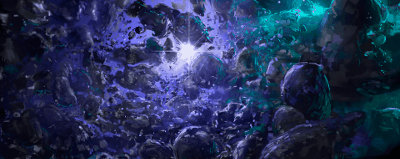
\includegraphics[width=\linewidth]{_img/places/asteroid-field.jpg}\\

Donc nos héros s’en vont chercher ce pour quoi ils sont venus, l’\nameref{sec:oubliette-de-dreypa} alias "la boite de Jebble". Mise à l’abri dans un champ d’astéroïdes par \nameref{sec:schurk-heren}.

Le champ d’astéroïde oblige les vaisseaux à sortir d’hyper-espace au large des coordonnées indiquées par Schurk. Dès la sortie, tous les voyants du \nameref{sec:nimbus} passent au rouge. En effet, ils ne sont pas seuls sur les lieux, une \nameref{sec:empire-corvette} de l’Empire est présente sur la zone. Quelques instants après leur arrivée, 4 \nameref{sec:tie-fighter} sont largués de la corvette et se dirigent vers le Nimbus pendant que la corvette s’engouffre dans le champ d’astéroïdes.

Un affrontement spatial s’engage entre le \nameref{sec:nimbus} et les 4 \nameref{sec:tie-fighter}. \textit{Les spécificités offensives et défensives des différents vaisseaux sont disponibles dans le \nameref{sec:bestiaire} et dans la section \nameref{sec:nimbus}}.\\

Une fois les 4 chasseurs explosés, les héros se précipitent (en principe) sur la zone où se trouve l’oubliette. Un cargo léger est en train de récupérer la cargaison de l’Uhumele quand le Nimbus arrive à portée de la corvette.

Les héros peuvent engager le combat, mais entre les dégâts encaissés contre les chasseurs et le fait que la corvette est mieux armée, le combat n’est pas égal. Ils peuvent prendre le cargo pour cible mais s’ils parviennent à l’exploser, la corvette utilisera un rayon tracteur pour récupérer la boite.

Au final, la corvette prendra la fuite sans demander son reste et les héros n’ont que leurs yeux pour pleurer.

\subsection{\'Epilogue}
C’est, pour une fois, un scénar qui ne se termine pas bien. On peut pas toujours gagner !

Pour l’XP, entre \textbf{2 et 3 XP} selon le jeu et la cohérence des joueurs.

\clearpage
\subsection{l’Uhumele}\label{sec:uhumele}
\noindent
\includegraphics[width=\textwidth]{_img/uhumele-pano.jpg}
\\

L’Uhumele est un vaisseau cargo de classe inconnue, actif notamment pendant et après la Guerre des Clones. Son capitaine est le Yarkora Schurk-Heren. On ignore quand et dans quelles conditions Schurk-Heren devint capitaine de l’Uhumele et comment son équipage le rejoignit. Ce qui est sûr, c’est qu’il a de bonnes raisons de détester la République et de craindre l’Empire qui lui succède.

L’Uhumele est avant tout un vaisseau de contrebande, comme un bon nombre de cargos en apparence en règle. De ce fait, il est doté d’un armement susceptible de pouvoir le sortir des situations délicates dans lesquelles il se fourre. L’une de ces armes est un bras rétractable situé sous le ventre de l’appareil, au bout duquel se trouve une petite tourelle blaster, ressemblant à celle des Canonnières clones. Bien que cette tourelle permette d’avoir un très vaste angle de tir, elle rend la situation du tireur précaire car très exposé. 

\hspace{5\baselineskip}
\noindent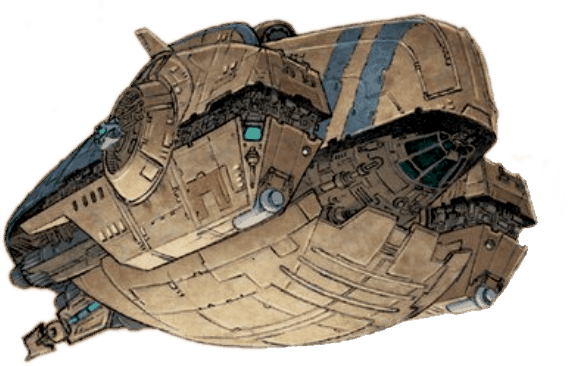
\includegraphics[width=0.7\textwidth]{_img/uhumele.png}

\newpage
\vspace*{11\baselineskip}
\subsubsection{Janks}\label{sec:uhumele-janks}
On sait très peu de choses sur le Phindien Janks, hormis le fait qu’il faisait partie de l’équipage de l’Uhumele en -19, au crépuscule de la Guerre des Clones. Son poste était celui d’ingénieur assistant de Ratty, le Tintinna ingénieur en chef. Janks n’était pas vraiment doué pour les plans complexes, c’est pourquoi il se contentait de suivre son équipage sans maugréer.

Pendant que le Capitaine Heren allait à la pêche aux renseignements, Janks se chargea d’acheter des provisions pour l’équipage. Alors qu’il retournait au vaisseau, il tomba nez à nez avec une patrouille impériale. Janks ne fut pas aussi rapide, d’autant plus qu’il avait été pris totalement par surprise. L’Empire se saisit de lui et le plaça en détention\ldots

Janks fut placé dans une cellule à bord d’un destroyer stellaire impérial et torturé pendant qu’on l’interrogerait sur l’équipage du Uhumele et sa cargaison.
